%
% Elliott Hudson College - Maths Booklet Template
% Created by: Ellis Dickinson
% Originally created on: May 3rd 2021
%
% LICENSE:
% This program is free software: you can redistribute it and/or modify
% it under the terms of the GNU General Public License as published by
% the Free Software Foundation, either version 3 of the License, or
% any later version.
%
% This program is distributed in the hope that it will be useful,
% but WITHOUT ANY WARRANTY; without even the implied warranty of
% MERCHANTABILITY or FITNESS FOR A PARTICULAR PURPOSE.  See the
% GNU General Public License for more details.
%
% You should have received a copy of the GNU General Public License
% along with this program. If not, see <https://www.gnu.org/licenses/>.
%
%
% IMPORTANT!!!!
% When compiling this document, please use XeLaTeX
% Other compilers do not support some of the features within this document.
%


\documentclass[fleqn]{article}

\setcounter{section}{1}                                             % Set the Unit Number (without Leading 0's)
\newcommand{\coursetitle}{AS Pure Mathematics (Year 1)}             % Set the Course Title
\newcommand{\bookletunittitle}{Algebraic expressions}               % Set the Unit Title
\newcommand{\bookletsubtitle}{Content last revised by: J Sherwood}  % Set the Subtitle
\newcommand{\unitprefix}{P}                                         % Set the Unit Prefix

% DO NOT MODIFY THIS FIILE
% ----------------------------------------------
\usepackage[dvipsnames]{xcolor}
\usepackage[a4paper, portrait, margin=1.9cm]{geometry}
\usepackage{titlesec}
\usepackage{tikz}\usetikzlibrary{shapes.misc}\usetikzlibrary{calc}
\usepackage{setspace}
\usepackage{fontspec}
\usepackage[most]{tcolorbox}
\usepackage{varwidth}
\usepackage[inline]{enumitem}
\usepackage{multicol}
\usepackage{fancyhdr}
\usepackage{booktabs, tabularx}
\usepackage{mathtools}
\usepackage{tasks}
\usepackage{anyfontsize}
\usepackage[export]{adjustbox}		% http://ctan.org/pkg/adjustbox




\newcounter{taskscounter}
\settasks{							% Multi-column enumeration
	style=enumerate,
	counter=taskscounter,
	label-width={22pt},
	item-indent={15pt},
	label-align=right,
	label=\textbf{\alph*},
	before-skip = -\parskip , 		% undo paragraph skip
  	after-skip = -\parskip , 		% undo paragraph skip
  	after-item-skip = -\parskip+1mm	% undo paragraph skip
%   debug=true 						% useful for fine-tuning or debugging
}



% Define dynamic titlebars for sections/exercises
\newlength{\sectionnumberwidth}
\newcommand\titlebar{\hspace*{-0.1cm}
	\tikz[baseline, trim right=3.1cm] {
		\settowidth{\sectionnumberwidth}{
			\pgfinterruptpicture
				\textbf{\sffamily\thesection.\thesubsection}
			\endpgfinterruptpicture
		}
	    \fill [cyan!25, rounded corners=0.15cm] (2.5cm,-1.28ex) rectangle (\textwidth-\sectionnumberwidth+2.65cm,2.615ex);
	    \node [
	        fill=blue!60!white,
	        text=white,
	        anchor= base east,
	        rounded rectangle,
	        inner sep = 2mm,
	        minimum height=3.89ex] at (3cm,0) {
	        {\bfseries\thesection.\thesubsection}
	    };
	}
}
\newcommand\exercisebar{\hspace*{-0.1cm}
	\tikz[baseline, trim right=3.1cm] {
		\settowidth{\sectionnumberwidth}{
			\pgfinterruptpicture
				\textbf{\sffamily\thesection.\thesubsubsection}
			\endpgfinterruptpicture
		}
	    \fill [red!25, rounded corners=0.15cm] (2.5cm,-1.265ex) rectangle (\textwidth-\sectionnumberwidth+2.65cm,2.64ex);
	    \node [
	        fill=cherryred!80!white,
	        text=white,
	        anchor= base east,
	        rounded rectangle,
	        inner sep = 2mm,
	        minimum height=3.9ex] at (3cm,0) {
	        {\bfseries\thesection\thesubsubsection}
	    };
	}
}

\newtcolorbox{mybox2}[2][]{
	enhanced,
	before skip=2mm,after skip=2mm,
	colback=black!5,
	colframe=black!50,
	boxrule=0.2mm,
	attach boxed title to top left={
		xshift=1cm,yshift*=1mm-\tcboxedtitleheight},
		varwidth boxed title*=-3cm,
		boxed title style={frame code={
            \path[fill=tcbcolback!30!black]
              ([yshift=-1mm,xshift=-1mm]frame.north west)
                arc[start angle=0,end angle=180,radius=1mm]
              ([yshift=-1mm,xshift=1mm]frame.north east)
                arc[start angle=180,end angle=0,radius=1mm];
            \path[left color=tcbcolback!60!black,right color=tcbcolback!60!black,
              middle color=tcbcolback!80!black]
              ([xshift=-2mm]frame.north west) -- ([xshift=2mm]frame.north east)
              [rounded corners=1mm]-- ([xshift=1mm,yshift=-1mm]frame.north east)
              -- (frame.south east) -- (frame.south west)
              -- ([xshift=-1mm,yshift=-1mm]frame.north west)
              [sharp corners]-- cycle;
            },interior engine=empty,
          },
	fonttitle=\sffamily\bfseries,
    title={#2},
    before upper = \sffamily,
    #1
}
          
\tcbset{%
    example/.style={%
        enhanced,
        breakable,
        rounded corners,
        toprule=0pt, rightrule=0pt, bottomrule=0pt, leftrule=1mm,
        colback=#1!5, colframe=#1!80!black, coltitle=#1!80!black,
        fonttitle=\bfseries\large\sffamily,
        detach title,
        before upper={\tcbtitle\quad},
        fontupper=\linespread{1.2}\selectfont
    },
    note/.style={%
        enhanced,
        breakable,
        separator sign none,
        rounded corners,
        toprule=0pt, rightrule=0pt, bottomrule=0pt, leftrule=1mm,
        colback=#1!5, colframe=#1!80!black, coltitle=#1!80!black,
        fonttitle=\bfseries\large,
        detach title,
        before upper={\sffamily\tcbtitle\quad\hspace{-2mm}},
        fontupper=\linespread{1.2}\selectfont
    }
}
\newtcbtheorem[auto counter]{examplebox}{Example}
{example=blue}{ex}
\newtcbtheorem{practice}{Independent Practice}
{example=practiceorange}{pr}
\newtcbtheorem{note}{#1\hspace{-1mm}}
{note=notecolor}{nt}



% Custom Colour Definitions
\definecolor{practiceorange}{RGB}{252, 191, 0}
\definecolor{notecolor}{RGB}{0, 0, 0}
\definecolor{cherryred}{RGB}{191,0,0}

\definecolor{ehclogoblue}{RGB}{0,187,211}
\definecolor{ehclogogray}{RGB}{33, 34, 33}
\definecolor{ehclogoorange}{RGB}{243, 108, 33}
\definecolor{separatorgray}{RGB}{210, 210, 210}



\setstretch{1.1} 										% Globally adjust bullet spacing
\setlength{\parindent}{0cm} 								% Removes paragraph indent
\setlength{\multicolsep}{6.0pt plus 2.0pt minus 1.5pt}	% Halves whitespace before multicol environment
\setlength\tabcolsep{0pt} 								% Removes default space between columns in table

% Change various spacings of bulleted/numbered lists
\setlist[itemize]{topsep=2pt, itemsep=-2pt}
\setlist[enumerate]{topsep=-2pt, partopsep=4mm, itemsep=0pt}

% Change spacing of aligned mathematics
\AtBeginDocument{
	\setlength\abovedisplayskip{3pt}
	%\setlength{\belowdisplayskip}{0pt}
	\setlength\belowdisplayskip{7pt}
	%\setlength{\belowdisplayshortskip}{0pt}
}


\setsansfont{AptiferSansPro}[
	Path = fonts/,
	Extension = .ttf,
    UprightFont = *-Regular,
    BoldFont = *-Medium
]



% Implement the custom titlebars
\titleformat{\section}{\large\sffamily}{\titlebar}{0.1cm}{}
\titleformat{\subsection}{\large\sffamily}{\titlebar}{0.1cm}{}
\titleformat{\subsubsection}{\large\sffamily}{\exercisebar}{0.1cm}{}



% Define the easier get functions for sections and subsections
\renewcommand*{\thesection}{\arabic{section}}
\renewcommand*{\thesubsection}{\arabic{subsection}}
\renewcommand*{\thesubsubsection}{\Alph{subsubsection}}
\newcommand\getcurrentref[1]{%
 \ifnumequal{\value{#1}}{0}
  {??}
  {\the\value{#1}}%
}
\newcommand{\exercise}{\subsubsection}



%Custom font size 'YUGE', larger than huge
\newcommand\YUGE{\fontsize{35}{35}\selectfont}

% Define custom footer
\fancypagestyle{plain}{
	\fancyhf{} % clear all header and footer fields
	\fancyfoot[OC]{ %right hand side
		\vspace{-0.7em}
		\hfill {\sffamily\raggedright {\color{separatorgray}\getcurrentref{page}} \\}\vspace{-1.6em}
		\begin{minipage}{.3\linewidth}
			\color{separatorgray}\rule{\linewidth}{0.4pt}
		\end{minipage}
		\begin{minipage}{.1\linewidth}
			\centering
			
\includegraphics[scale=0.4]{images/ehc-brand-separator-icon}
		\end{minipage}
		\begin{minipage}{.3\linewidth}
			\color{separatorgray}\rule{\linewidth}{0.4pt}
		\end{minipage}
	}
	\fancyfoot[EC]{ %left hand side
		\vspace{-0.7em}
		{\sffamily\raggedright {\color{separatorgray}\getcurrentref{page}} \\}\vspace{-1.6em}
		\begin{minipage}{.3\linewidth}
			\color{separatorgray}\rule{\linewidth}{0.4pt}
		\end{minipage}
		\begin{minipage}{.1\linewidth}
			\centering
			
\includegraphics[scale=0.4]{images/ehc-brand-separator-icon}
		\end{minipage}
		\begin{minipage}{.3\linewidth}
			\color{separatorgray}\rule{\linewidth}{0.4pt}
		\end{minipage}
	}

	\renewcommand{\headrulewidth}{0pt}
	\renewcommand{\footrulewidth}{0pt}
}
\pagestyle{plain}



% Function for adding vspace above underbrace
\newcommand*\addunderbracespace[1]{\vrule width0pt height0pt depth#1\relax}


\newcommand{\formattedunittitle}{Unit P\getcurrentref{section}}

\bluetheme


% TODO Document Begins
\begin{document}
% DO NOT MODIFY THIS FIILE
% ----------------------------------------------
% Title Page
% ----------------------------------------------
% Modified from a post from a post by ModyTex
% https://www.reddit.com/r/LaTeX/comments/faij1n/my_first_cover_page_done_in_latex_is_it/
% ----------------------------------------------
\pagestyle{empty}
\begin{tikzpicture}[overlay,remember picture]
    \begin{scope}[transform canvas ={rotate around ={45:($(current page.north)+(-1.5,-3)$)}}]
    \shade[rounded corners=12pt, left color=gray!80, right color=gray!80] ($(current page.north)+(-2,-6.7)$) rectangle ++(9,0.8);
    \end{scope}

    \begin{scope}[transform canvas ={rotate around ={45:($(current page.north)+(-3,-8)$)}}]
    \shade[rounded corners=20pt, left color=lightgray!80, right color=lightgray!80] ($(current page.north)+(2.5,-8)$) rectangle ++(15,1.35);
    \end{scope}

    \begin{scope}[transform canvas ={rotate around ={45:($(current page.north west)+(4,-15.5)$)}}]
    \shade[rounded corners=20pt, left color=ehclogoorange, right color=ehclogoorange] ($(current page.north west)+(15,-16)$) rectangle ++(20,1.5);
    \end{scope}

    \begin{scope}[transform canvas ={rotate around ={45:($(current page.north west)+(13,-10)$)}},]
    \shade[rounded corners=18pt, left color=ehclogoblue ,right color=ehclogoblue] ($(current page.north west)+(14.5,-10)$) rectangle ++(15,1.3);
    \end{scope}

    \begin{scope}[transform canvas ={rotate around ={45:($(current page.north west)+(18,-8)$)}},]
    \shade[rounded corners=8pt, left color=ehclogogray, right color=ehclogogray] ($(current page.north west)+(18.5,-8)$) rectangle ++(15,0.6);
    \end{scope}

    \begin{scope}[transform canvas ={rotate around ={45:($(current page.north west)+(19,-5.65)$)}},]
    \shade[rounded corners=12pt, left color=lightgray, right color=lightgray] ($(current page.north west)+(15.5,-5.65)$) rectangle ++(15,0.8);
    \end{scope}

    \begin{scope}[transform canvas ={rotate around ={45:($(current page.north west)+(20,-9)$)}}]
    \shade[rounded corners=15pt, left color=ehclogoorange, right color=ehclogoorange] ($(current page.north west)+(20,-8.4)$) rectangle ++(14,1.1);
    \end{scope}
\end{tikzpicture}

\vspace{-0.5cm}

\includegraphics{images/branding/brand-logo-vector}

\vspace{8.5cm}
\begin{minipage}{\textwidth}
    \sffamily

    \vspace{2mm}
    {\YUGE \raggedleft\bookletunittitle\\}

    \vspace{1mm}
    {\huge \raggedleft\coursetitle { }-- \formattedunittitle\\}

    \vspace{2mm}
    {\small \raggedleft\bookletsubtitle\\}
\end{minipage}
\vfill
% Key Information
% ----------------------------------------------

\begin{adjustbox}{valign=b}
	\begin{minipage}{.85\textwidth}
		\begin{mybox2}[colbacktitle=green]{Key Information}
			\textbf{Key Formulae:}
			\[
			\begin{aligned}
				x^a \times x^b &= x^{a+b} \\
				x^a \div x^b &= x^{a-b} \\
				(x^a)^b &= x^{ab} \\
				x^{-n} &= \dfrac{1}{x^n} \\
				x^{\tfrac{1}{n}} &= \sqrt[\textstyle{^n}]{x} \\
				a^2 - b^2 &= (a-b)(a+b)
			\end{aligned}
			\]

			\textbf{Key Terms:}
			\begin{itemize}
				\item \textbf{Expanding Brackets:} Multiplying brackets out
				\item \textbf{Factorising Brackets:} Putting expressions back into brackets
				\item \textbf{Surd:} A root of a number which can't be written as a whole number or fraction
				\item \textbf{Rationalising Denominator:} Removing the surd from the bottom of the fraction
			\end{itemize}
		\end{mybox2}
	\end{minipage}
\end{adjustbox}
\begin{minipage}[b]{.13\textwidth}
	\sffamily
	Solution Bank:
	\vspace{1mm}\linebreak
	
\includegraphics[scale=0.15, valign=b]{images/link-to-y1-sol-bank}
\end{minipage}



\begin{keyinformation}{images/links/maths/pure/year-1}
    \textbf{Key Formulae:}
    \begin{align*}
        x^a \times x^b &= x^{a+b}                    \\
        x^a \div x^b &= x^{a-b}                      \\
        (x^a)^b &= x^{ab}                            \\
        x^{-n} &= \dfrac{1}{x^n}                     \\
        x^{\tfrac{1}{n}} &= \sqrt[\textstyle{^n}]{x} \\
        a^2 - b^2 &= (a-b)(a+b)
    \end{align*}

    \textbf{Key Terms:}
    \begin{itemize}
        \item \textbf{Expanding Brackets:} Multiplying brackets out
        \item \textbf{Factorising Brackets:} Putting expressions back into brackets
        \item \textbf{Surd:} A root of a number which can't be written as a whole number or fraction
        \item \textbf{Rationalising Denominator:} Removing the surd from the bottom of the fraction
    \end{itemize}
\end{keyinformation}



\newpage
\pagestyle{attribution}



% TODO Links to the Big Picture
\begin{mybox2}[colbacktitle=WildStrawberry]{Links to the Big Picture}
    \begin{enumerate}[label*=\bfseries P\arabic*., leftmargin=*]
        \setcounter{enumi}{\getcurrentref{section}-1}
        \item \textbf{\bookletunittitle}
        \begin{enumerate}[label*=\bfseries\arabic*]
            % Unit Components Go Here
            \item Index Laws
            \item Expanding Brackets
            \item Factorising
            \item Negative and fractional indices
            \item Surds
            \item Rationalising Denominators
        \end{enumerate}
    \end{enumerate}
    \begin{tabularx}{\dimexpr\textwidth}{X@{\hskip6pt}X}
        {
            Develops:
            \begin{itemize}
                \item GCSE algebraic manipulation
            \end{itemize}
        } & {
            Leads to:
            \begin{itemize}
                \item P2 -- Quadratics
                \item P6 -- Algebraic Methods
                \item P9 -- Integration
                \item P12 -- Differentiation
                \item P13 -- Integration
            \end{itemize}
        }
    \end{tabularx}
\end{mybox2}

\begin{note*}{Exam Question}{}
    \rmfamily
    \begin{enumerate}[label=\textbf{\alph*}]
        \item Write $\sqrt{45}$ in the form $a\sqrt{5}$, where $a$ is an integer.\hfill\textbf{(1 mark)}
        \item Express $\cfrac{2(3+\sqrt{5})}{(3-\sqrt{5})}$ in the form $b+c\sqrt{5}$, where $b$ and $c$ are integers. \hfill\textbf{(5 marks)}
    \end{enumerate}

\end{note*}

\newpage
\pagestyle{branded}
\setcounter{page}{1}




\begin{minipage}[t]{.85\textwidth}
        \sffamily\setstretch{1.1}
        \bfseries\YUGE\raggedright\bookletunittitle\\
\end{minipage}
\begin{minipage}[t]{.15\textwidth}
        \sffamily
        \bfseries\YUGE\raggedleft\getcurrentref{section}
\end{minipage}

\begin{mybox2}[colbacktitle=green]{Overview}
    After completing this chapter you should be able to:
    \begin{itemize}
        \item Multiply and divide integer powers
        \item Expand a single term over brackets and collect like terms
        \item Expand the product of two or three expressions
        \item Factorise linear, quadratic and simple cubic expressions
        \item Know and use the laws of Indices
        \item Simplify and use the rules of surds
        \item Rationalise denominators
    \end{itemize}
\end{mybox2}




\lesson{Index Laws}
\textbullet{You can use the laws of indices to simplify powers of the same base.}
\begin{itemize}
    \item $a^m \times a^n = a^{m+n}$
    \item $a^m \div a^n = a^{m-n}$
    \item $(a^m)^n = a^{mn}$
    \item $(ab)^n = a^nb^n$
\end{itemize}




\begin{examplebox}{}{}
    \\ % TODO Example 1
    Simplify these expressions:                        \\
    \textbf{a}\hspace{2mm} $x^2 \times x^5$            \hspace{7mm} \
    \textbf{b}\hspace{2mm} $2r^2 \times 3r^3$          \hspace{7mm} \
    \textbf{c}\hspace{2mm} $\dfrac{b^7}{b^4}$          \hspace{7mm} \
    \textbf{d}\hspace{2mm} $6x^5 \div 3x^3$            \hspace{7mm} \
    \textbf{e}\hspace{2mm} $(a^3)^3 \times 2a^2$       \hspace{7mm} \
    \textbf{f}\hspace{2mm} $(3x^2)^3 \div x^4$
\end{examplebox}

\newpage




\begin{table}[!ht]
    \vspace{-4mm}
    \begin{tabularx}{\dimexpr\textwidth}{X@{\hskip6pt}p{2.5in}}
        \vspace{-5mm}
        \begin{examplebox}{}{}
            \\ % TODO Example 2
            Expand these expressions and simplify if possible:
            \begin{multicols}{2}
                \textbf{a}\hspace{2mm} $-3x(7x-4)$          \newline
                \textbf{c}\hspace{2mm} $4x(3x-2x^2+5x^3)$
                \columnbreak
                \newline
                \textbf{b}\hspace{2mm} $y^2(3-2y^3)$        \newline
                \textbf{d}\hspace{2mm} $2x(5x+3)-5(2x+3)$
            \end{multicols}
        \end{examplebox} & \begin{note*}{Watch Out}{}
            A minus sign outside brackets changes the sign of every term inside the brackets.
        \end{note*}
    \end{tabularx} 
\end{table}
\vspace{8.5cm}

\begin{examplebox}{}{}
    \\ % TODO Example 3
    Simplify these expressions:\vspace{2mm}            \\
    \textbf{a}\hspace{2mm} $\dfrac{x^7+x^4}{x^3}$      \hspace{7mm} \
    \textbf{b}\hspace{2mm} $\dfrac{3x^2-6x^5}{2x}$     \hspace{7mm} \
    \textbf{c}\hspace{2mm} $\dfrac{20x^7+15x^3}{5x^2}$
\end{examplebox}

\vfill
\begin{practice*}{Exercise 1A}{}
\end{practice*}
\newpage


\lesson{Expanding Brackets}
\begin{mybox2}[colbacktitle=green]{Finding the product}
    To find the \textbf{product} of two expressions you \textbf{multiply} each term in one expression by each term in the other expression.



\tikzset{every picture/.style={line width=0.75pt}} %set default line width to 0.75pt
\tikzstyle{every node}=[font=\footnotesize]


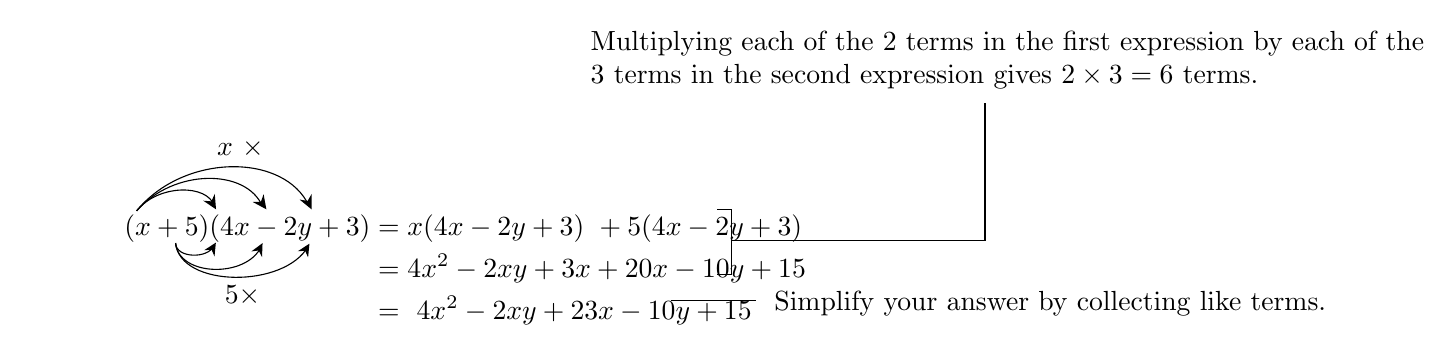
\begin{tikzpicture}[x=0.75pt,y=0.75pt,yscale=-0.75,xscale=0.75]
    \path (10,208); %set diagram left start at 10, and has height of 215 - used for diagram positioning

    %Curve Lines [id:da7159687887985733]
    \draw    (80,132.33) .. controls (93.76,115) and (125.7,115) .. (129.84,129.21) ;
    \draw [shift={(131,131.33)}, rotate = 239.62] [fill={rgb, 255:red, 0; green, 0; blue, 0 }  ][line width=0.08]  [draw opacity=0] (8.93,-4.29) -- (0,0) -- (8.93,4.29) -- (5.93,0) -- cycle    ;
    %Curve Lines [id:da8632837875960184]
    \draw    (80,132.33) .. controls (103.84,105) and (150.42,105) .. (160.82,129.38) ;
    \draw [shift={(163.33,131.33)}, rotate = 233.97] [fill={rgb, 255:red, 0; green, 0; blue, 0 }  ][line width=0.08]  [draw opacity=0] (8.93,-4.29) -- (0,0) -- (8.93,4.29) -- (5.93,0) -- cycle    ;
    %Curve Lines [id:da17709854996093832]
    \draw    (80,132.33) .. controls (110.46,95) and (175.3,95) .. (190.82,129.37) ;
    \draw [shift={(192.33,131.33)}, rotate = 245] [fill={rgb, 255:red, 0; green, 0; blue, 0 }  ][line width=0.08]  [draw opacity=0] (8.93,-4.29) -- (0,0) -- (8.93,4.29) -- (5.93,0) -- cycle    ;
    %Shape: Right Angle [id:dp13326247026484794]
    \draw   (625,63.33) -- (625,151.33) -- (462,151.33) ;
    %Shape: Right Angle [id:dp5046670172690588]
    \draw   (462,151.33) -- (462,173.33) -- (453,173.33) ;
    %Shape: Right Angle [id:dp09935594472445719]
    \draw   (462,151.33) -- (462,131.33) -- (453,131.33) ;
    %Straight Lines [id:da5023172987675482]
    \draw    (423,190) -- (478,190) ;
    %Curve Lines [id:da29076012404221396]
    \draw    (105,153) .. controls (105.41,163) and (125.75,163) .. (129.24,155.15) ;
    \draw [shift={(130.89,152.72)}, rotate = 481.22] [fill={rgb, 255:red, 0; green, 0; blue, 0 }  ][line width=0.08]  [draw opacity=0] (8.04,-3.86) -- (0,0) -- (8.04,3.86) -- (5.34,0) -- cycle    ;
    %Curve Lines [id:da6548003424940994]
    \draw    (105,153) .. controls (106.9,174.61) and (150.42,175.67) .. (160,155.35) ;
    \draw [shift={(160.89,153.06)}, rotate = 477.9] [fill={rgb, 255:red, 0; green, 0; blue, 0 }  ][line width=0.08]  [draw opacity=0] (8.04,-3.86) -- (0,0) -- (8.04,3.86) -- (5.34,0) -- cycle    ;
    %Curve Lines [id:da913578758781056]
    \draw    (105,153) .. controls (108,181.98) and (175.3,182.07) .. (190.18,155) ;
    \draw [shift={(191,153.39)}, rotate = 481.16] [fill={rgb, 255:red, 0; green, 0; blue, 0 }  ][line width=0.08]  [draw opacity=0] (8.04,-3.86) -- (0,0) -- (8.04,3.86) -- (5.34,0) -- cycle    ;

    % Text Node
    \draw (130,85) node [anchor=north west][inner sep=0.75pt]    {$x\ \times $};
    % Text Node
    \draw (370,15) node [anchor=north west][inner sep=0.75pt]   [align=left] {Multiplying each of the 2 terms in the first expression by each of the\\3 terms in the second expression gives $\displaystyle 2\times 3=6$ terms.};
    % Text Node
    \draw (488,182) node [anchor=north west][inner sep=0.75pt]   [align=left] {Simplify your answer by collecting like terms.};
    % Text Node
    \draw (55.67,131.4) node [anchor=north west][inner sep=0.75pt]    {$ \begin{array}{l}
    \ \begin{aligned}
    ( x+5)( 4x-2y+3) & =x( 4x-2y+3) \ +5( 4x-2y+3)\\
     & =4x^{2} -2xy+3x+20x-10y+15\\
     & =\ 4x^{2} -2xy+23x-10y+15
    \end{aligned}\\
    \end{array}$};
    % Text Node
    \draw (135,178.4) node [anchor=north west][inner sep=0.75pt]    {$5\times $};
    \end{tikzpicture}
\end{mybox2}


\begin{examplebox}{}{}
    \\ % TODO Example 4
    Expand these expressions and simplify if possible:  \\
    \textbf{a}\hspace{2mm} $(x+5)(x+2)$                 \hspace{7mm} \
    \textbf{b}\hspace{2mm} $(x-2y)(x^2+1)$              \hspace{7mm} \
    \textbf{c}\hspace{2mm} $(x-y)^2$                    \hspace{7mm} \
    \textbf{d}\hspace{2mm} $(x+y)(3x-2y-4)$             \hspace{7mm} \
\end{examplebox}
\newpage


\begin{examplebox}{}{}
    \\ % TODO Example 5
    Expand these expressions and simplify if possible:  \\
    \textbf{a}\hspace{2mm} $x(2x+3)(x-7)$               \hspace{7mm} \
    \textbf{b}\hspace{2mm} $x(5x-3y)(2x-y+4)$           \hspace{7mm} \
    \textbf{c}\hspace{2mm} $(x-4)(x+3)(x+3)$            \hspace{7mm} \
\end{examplebox}
\vfill
\begin{practice*}{Exercise 1B}{}
\end{practice*}
\newpage




\lesson{Factorising}
\begin{mybox2}[colbacktitle=green]{}
    \begin{multicols}{2}
        You can write expressions as a \textbf{product of their factors.}\\\\
        \textbullet{ }\textbf{Factorising is the opposite of expanding brackets.}
        \newline
        \columnbreak
        \hspace{2cm}
        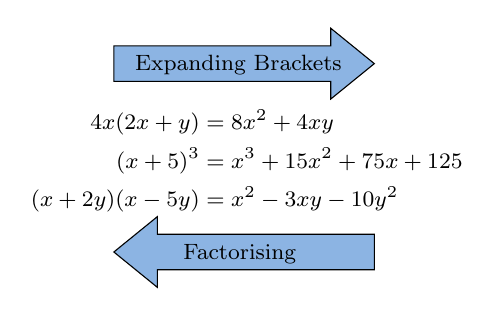
\begin{tikzpicture}[x=0.75pt,y=0.75pt,yscale=-0.75,xscale=0.75]
            \tikzstyle{every node}=[font=\footnotesize]
            %uncomment if require: \path (0,186); %set diagram left start at 0, and has height of 186

            %Right Arrow [id:dp33217389058940294]
            \draw  [color={rgb, 255:red, 0; green, 0; blue, 0 }  ,draw opacity=1 ][fill={rgb, 255:red, 140; green, 180; blue, 227 }  ,fill opacity=1 ] (67,20.38) -- (206.33,20.38) -- (206.33,9) -- (234.33,31.75) -- (206.33,54.5) -- (206.33,43.13) -- (67,43.13) -- cycle ;
            %Left Arrow [id:dp9804470166273318]
            \draw  [color={rgb, 255:red, 0; green, 0; blue, 0 }  ,draw opacity=1 ][fill={rgb, 255:red, 140; green, 180; blue, 227 }  ,fill opacity=1 ] (234.33,141.38) -- (95,141.38) -- (95,130) -- (67,152.75) -- (95,175.5) -- (95,164.13) -- (234.33,164.13) -- cycle ;

            % Text Node
            \draw (12,59.4) node [anchor=north west][inner sep=0.75pt]    {$\begin{aligned}
            4x( 2x+y) & =8x^{2} +4xy\\
            ( x+5)^{3} & =x^{3} +15x^{2} +75x+125\\
            ( x+2y)( x-5y) & =x^{2} -3xy-10y^{2}
            \end{aligned}$};
            % Text Node
            \draw (79,24.5) node [anchor=north west][inner sep=0.75pt]   [align=left] {Expanding Brackets};
            % Text Node
            \draw (110,146) node [anchor=north west][inner sep=0.75pt]   [align=left] {Factorising};
        \end{tikzpicture}
    \end{multicols}
\end{mybox2}

\begin{examplebox}{}{}
    \\ % TODO Example 6
    Factorise these expressions completely:    \\
    \textbf{a}\hspace{2mm} $3x+9$              \hspace{7mm} \
    \textbf{b}\hspace{2mm} $x^2-5x$            \hspace{7mm} \
    \textbf{c}\hspace{2mm} $8x^2+20x$          \hspace{7mm} \
    \textbf{d}\hspace{2mm} $9x^2y+15^xy^2$     \hspace{7mm} \
    \textbf{e}\hspace{2mm} $3x^2-9xy$          \hspace{7mm} \
\end{examplebox}

\vfill
\begin{mybox2}[colbacktitle=green]{}
    \begin{multicols}{2}
        \textbullet { }\textbf{A quadratic expression had the form $ax^2+bx+c$ where $a$, $b$ and $c$ are real numbers and $a\neq0$.}
        \columnbreak
        \newline
        \textbf{Notation: }Real numbers are all the positive and\\ negative numbers, or zero, including fractions and surds.
    \end{multicols}
    \vspace{2mm}
    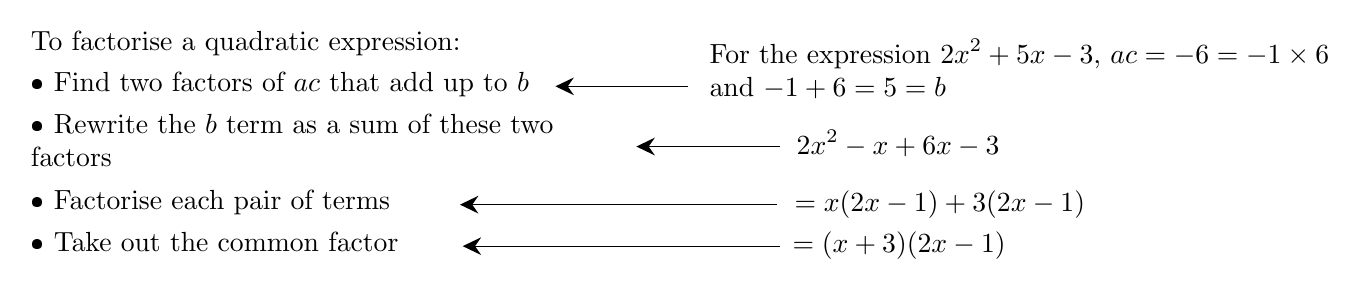
\begin{tikzpicture}[x=0.75pt,y=0.75pt,yscale=-1,xscale=1]
        %uncomment if require: \path (0,300); %set diagram left start at 0, and has height of 300

        %Straight Lines [id:da16583134338090377]
        \draw    (338,51) -- (277,51) ;
        \draw [shift={(274,51)}, rotate = 360] [fill={rgb, 255:red, 0; green, 0; blue, 0 }  ][line width=0.08]  [draw opacity=0] (8.93,-4.29) -- (0,0) -- (8.93,4.29) -- (5.93,0) -- cycle    ;
        %Straight Lines [id:da7338024028726267]
        \draw    (382,80) -- (316,80) ;
        \draw [shift={(313,80)}, rotate = 360] [fill={rgb, 255:red, 0; green, 0; blue, 0 }  ][line width=0.08]  [draw opacity=0] (8.93,-4.29) -- (0,0) -- (8.93,4.29) -- (5.93,0) -- cycle    ;
        %Straight Lines [id:da6781583727070806]
        \draw    (380.67,108) -- (232,108) ;
        \draw [shift={(228,108)}, rotate = 360] [fill={rgb, 255:red, 0; green, 0; blue, 0 }  ][line width=0.08]  [draw opacity=0] (8.93,-4.29) -- (0,0) -- (8.93,4.29) -- (5.93,0) -- cycle    ;
        %Straight Lines [id:da4054867925968648]
        \draw    (382,128) -- (232,128) ;
        \draw [shift={(229.33,128)}, rotate = 360] [fill={rgb, 255:red, 0; green, 0; blue, 0 }  ][line width=0.08]  [draw opacity=0] (8.93,-4.29) -- (0,0) -- (8.93,4.29) -- (5.93,0) -- cycle    ;

        % Text Node
        \draw (20,23) node [anchor=north west][inner sep=0.75pt]   [align=left] {To factorise a quadratic expression:};
        \draw (20,43) node [anchor=north west][inner sep=0.75pt]   [align=left] {\mbox{\textbullet} Find two factors of $\displaystyle ac$ that add up to $\displaystyle b$};
        \draw (20,63) node [anchor=north west][inner sep=0.75pt]   [align=left] {\mbox{\textbullet} Rewrite the $\displaystyle b$ term as a sum of these two\\factors};
        \draw (20,100) node [anchor=north west][inner sep=0.75pt]   [align=left] {\mbox{\textbullet} Factorise each pair of terms};
        \draw (20,120) node [anchor=north west][inner sep=0.75pt]   [align=left] {\mbox{\textbullet} Take out the common factor};


        % Text Node
        \draw (347,27) node [anchor=north west][inner sep=0.75pt]   [align=left] {For the expression $\displaystyle 2x^{2} +5x-3$, $\displaystyle ac = -6 = -1 \displaystyle \times 6$\\and $-1 +6 = 5 =  b$};
        % Text Node
        \draw (389,71) node [anchor=north west][inner sep=0.75pt]   [align=left] {$\displaystyle 2x^{2} -x+6x-3$};
        % Text Node
        \draw (388,100) node [anchor=north west][inner sep=0.75pt]    {$=x( 2x-1) +3( 2x-1)$};
        % Text Node
        \draw (387,120) node [anchor=north west][inner sep=0.75pt]    {$=( x+3)( 2x-1)$};
    \end{tikzpicture}
    \begin{multicols}{2}
        \textbullet { }$x^2-y^2=(x+y)(x-y)$
        \columnbreak
        \newline
        \textbf{Notation: }An expression in the form $x^2-y^2$ is called the \textbf{difference} of two sqaures.
    \end{multicols}
\end{mybox2}
\newpage


\begin{examplebox}{}{}
    \\ % TODO Example 7
    Factorise: \\
    \textbf{a}\hspace{2mm} $x^2-5x-6$            \hspace{7mm} \
    \textbf{b}\hspace{2mm} $x^2+6x+8$            \hspace{7mm} \
    \textbf{c}\hspace{2mm} $6x^2-11x-10$         \hspace{7mm} \
    \textbf{d}\hspace{2mm} $x^2-25$              \hspace{7mm} \
    \textbf{e}\hspace{2mm} $4x^2-9y^2$           \hspace{7mm}
\end{examplebox}


\vspace{9cm}
\begin{examplebox}{}{}
    \\ % TODO Example 8
    Factorise completely:                        \\
    \textbf{a}\hspace{2mm} $x^3-2x^2$            \hspace{7mm} \
    \textbf{b}\hspace{2mm} $x^3-25x$             \hspace{7mm} \
    \textbf{c}\hspace{2mm} $x^3+3x^2-10x$        \hspace{7mm}
\end{examplebox}

\vfill
\begin{practice*}{Exercise 1C}{}
\end{practice*}
\newpage

\lesson{Negative and fractional indices}
\vspace{-6mm}
\begin{table}[!ht]
    \begin{tabularx}{\dimexpr\textwidth}{X@{\hskip6pt}p{2.5in}}
       \begin{mybox2}[colbacktitle=green]{}
           Indices can be negative or fractions.\\
           \\
           $x^{\textstyle\frac{1}{2}}\times x^{\textstyle\frac{1}{2}} = x^{\textstyle\frac{1}{2}+\textstyle\frac{1}{2}}=x^1=x$
           \vspace{3mm}\\
        similarly $\underbrace{\addunderbracespace{1ex}x^{\textstyle\frac{1}{n}} \times x^{\textstyle\frac{1}{n}} \times ... \times x^{\textstyle\frac{1}{n}}}_{n \text{ terms}} = x^{\textstyle\frac{1}{n}+\textstyle\frac{1}{n}+...+\textstyle\frac{1}{n}}+x^1=x$

        \vspace{3mm}
        \textbullet{} You can use the laws of indices with any rational power.
        \begin{itemize}
            \item $a^{\textstyle\frac{1}{m}}=\sqrt[\textstyle{^m}]{a}$     \vspace{-1mm}
            \item $a^{\textstyle\frac{n}{m}}=\sqrt[\textstyle{^m}]{a^n}$   \vspace{-1mm}
            \item $a^{-m}=\dfrac{1}{a^m}$                                  \vspace{-1.5mm}
            \item $a^0=1$
        \end{itemize}


         \end{mybox2} & \begin{note*}{Notation}{}
            \vspace{0.5mm}Rational numbers\\are those that can be written $\dfrac{a}{b}$\\ where $a$ and $b$ are integers.
        \end{note*}
        \vspace{-5mm}
        \begin{note*}{Notation}{}
            \vspace{0.5mm}$a^{\textstyle\frac{1}{2}}=\sqrt{a}$ is the \\positive square root of $a$. \\For example $9^{\textstyle\frac{1}{2}}=\sqrt{9}=3$ \\but $9^{\textstyle\frac{1}{2}}\neq-3$.
        \end{note*}
    \end{tabularx}
    \vspace{-4mm}
\end{table}

\begin{examplebox}{}{}
    \\ % TODO Example 9
    Simplify: \\
    \textbf{a}\hspace{2mm} $\dfrac{x^3}{x^{-3}}$                                          \hspace{7mm} \
    \textbf{b}\hspace{2mm} $x^{\textstyle\frac{1}{2}}\times x^{\textstyle\frac{3}{2}}$    \hspace{7mm} \
    \textbf{c}\hspace{2mm} $(x^3)^{\textstyle\frac{2}{3}}$                                \hspace{7mm} \
    \textbf{d}\hspace{2mm} $2x^{1.5}\div 4x^{-0.25}$                                      \hspace{7mm} \
    \textbf{e}\hspace{2mm} $\sqrt[\textstyle{^3}]{125x^6}$                                \hspace{7mm}
\end{examplebox}


\newpage
\begin{examplebox}{}{}
    \\ % TODO Example 10
    Evaluate:
    \vspace{1.5mm}\\
    \textbf{a}\hspace{2mm} $9^{\textstyle\frac{1}{2}}$         \hspace{15mm} \
    \textbf{b}\hspace{2mm} $64^{\textstyle\frac{1}{3}}$        \hspace{15mm} \
    \textbf{c}\hspace{2mm} $49^{\textstyle\frac{3}{2}}$        \hspace{15mm} \
    \textbf{d}\hspace{2mm} $25^{-\textstyle\frac{3}{2}}$       \hspace{15mm}
\end{examplebox}
\vspace{9cm}
\begin{examplebox}{}{}
    \\ % TODO Example 11
    Factorise completely:
    \vspace{1.5mm}\\
    \textbf{a}\hspace{2mm} $y^{\textstyle\frac{1}{2}}$        \hspace{15mm} \
    \textbf{b}\hspace{2mm} $4y^{-1}$                          \hspace{7mm}
\end{examplebox}

\vfill
\begin{practice*}{Exercise 1D}{}
\end{practice*}
\newpage



\lesson{Surds}
\vspace{-6mm}

\begin{table}[!ht]
    \begin{tabularx}{\dimexpr\textwidth}{X@{\hskip6pt}p{2.5in}}
        \begin{mybox2}[colbacktitle=green]{}
            If $n$ is an integer that is \textbf{not} a square number, then any multiple of $\sqrt{n}$ is called a surd.\\
            Examples of surds are: $\sqrt{2}$, $\sqrt{19}$ and $5\sqrt{2}$

            \vspace{2mm}

            Surds are examples of \textbf{irrational numbers}. \\The decimal expansion of a surd is never-ending and never\\ repeats, for example $\sqrt{2}$ = 1.414213562...

            \vspace{2mm}
            You can use surds to write exact answers to calculations.
            \vspace{2mm}

            \textbullet\space You can manipulate surds using these rules:
            \begin{itemize}
                \item $\sqrt{\strut ab}=\sqrt{\strut a}\times\sqrt{\strut b}$
                \item $\sqrt{\cfrac{a}{b}}=\dfrac{\sqrt{a}}{\sqrt{b}}$
            \end{itemize}


        \end{mybox2} & \begin{note*}{Notation}{}
            \vspace{0.5mm}Irrational numbers \\\vspace{1mm}cannot be written in the form $\dfrac{a}{b}$ where $a$ and $b$ are integers.
            Surds are examples of \textbf{irrational numbers}.
        \end{note*}
    \end{tabularx}
    \vspace{-4mm}
\end{table}
\begin{examplebox}{}{}
    \\ % TODO Example 12
    Simplify: \\
    \textbf{a}\hspace{2mm} $\sqrt{12}$                           \hspace{15mm} \
    \textbf{b}\hspace{2mm} $\cfrac{\sqrt{20}}{2}$                \hspace{15mm} \
    \textbf{c}\hspace{2mm} $5\sqrt{6}-2\sqrt{24}+\sqrt{294}$     \hspace{15mm}
\end{examplebox}

\vspace{5cm}
\begin{examplebox}{}{}
    \\ % TODO Example 13
    Simplify: \\
    \textbf{a}\hspace{2mm} $\sqrt{2}(5-\sqrt{3})$        \hspace{20mm} \
    \textbf{b}\hspace{2mm} $(2-\sqrt{3})(5+\sqrt{3})$    \hspace{20mm}
\end{examplebox}

\vfill
\begin{practice*}{Exercise 1E}{}
\end{practice*}
\newpage




\lesson{Rationalising denominators}
\begin{mybox2}[colbacktitle=green]{}
    If a fraction has a surd in the denominator, it is sometimes useful to \textbf{rearrange} it so that the denominator is a rational number. This is called rationalising the denominator.
    \vspace{2mm}

    \textbullet\space The rules to rationalise denominators are:\vspace{-2mm}
    \begin{itemize}
        \setlength{\itemsep}{-3pt}%
        \item For fractions in the form $\cfrac{1}{\sqrt{a}}$, multiply the numerator and denominator by $\sqrt{a}$.
        \item For fractions in the form $\cfrac{1}{a+\sqrt{a}}$, multiply the numerator and denominator by $a-\sqrt{a}$.
        \item For fractions in the form $\cfrac{1}{a-\sqrt{a}}$, multiply the numerator and denominator by $a+\sqrt{a}$.
    \end{itemize}

\end{mybox2}
\begin{examplebox}{}{}
    \\ % TODO Example 14
    Rationalise the denominator of: \\
    \textbf{a}\hspace{2mm} $\cfrac{1}{\sqrt{3}}$                      \hspace{20mm} \
    \textbf{b}\hspace{2mm} $\cfrac{1}{3+\sqrt{2}}$                    \hspace{20mm} \
    \textbf{c}\hspace{2mm} $\cfrac{\sqrt{5}+\sqrt{2}}{3+\sqrt{2}}$    \hspace{20mm} \
    \textbf{d}\hspace{2mm} $\cfrac{1}{(1-\sqrt{3})^2}$                \hspace{20mm} \
\end{examplebox}

\vfill
\begin{practice*}{Exercise 1F}{}
\end{practice*}
\newpage

\begin{mybox2}[colbacktitle=green]{Summary of key points}
    \begin{enumerate}
        \item You can use the laws of indices to simplify powers of the \textbf{same base}.
            \begin{multicols}{2}
                \begin{itemize}
                    \item $a^m\times a^n = a^{m+n}$
                    \item $(a^m)^n = a^{mn}$
                \end{itemize}
                \columnbreak
                \begin{itemize}
                    \setlength{\itemsep}{-3pt}
                    \item $a^m\div a^n = a^{m-n}$
                    \item $(ab)^n = a^nb^n$
                \end{itemize}
            \end{multicols}
        \item Factorising is the opposite of expanding brackets.
        \item A quadratic expression has the form $ax^2+bx+c$ where $a$, $b$, and $c$ are real numbers and $a\neq0$.
        \item $x^2-y^2=(x+y)(x-y)$
        \item You can use the laws of indices with any rational power.
            \begin{multicols}{2}
                \begin{itemize}
                    \item $a^{\textstyle\frac{1}{m}}=\sqrt[\textstyle{^m}]{\strut a}$
                    \item $a^{-m}=\dfrac{1}{a^m}$
                \end{itemize}
                \columnbreak
                \begin{itemize}
                    \setlength{\itemsep}{-3pt}
                    \item $a^{\textstyle\frac{n}{m}}=\sqrt[\textstyle{^m}]{\strut a^n}$
                    \item $a^0 = 1$
                \end{itemize}
            \end{multicols}
        \item You can manipulate surds using the rules:
            \begin{multicols}{2}
                \vspace{2mm}
                \begin{itemize}
                    \item $\sqrt{\strut ab}=\sqrt{\strut a}\times\sqrt{\strut b}$
                \end{itemize}
                \columnbreak
                \begin{itemize}
                    %\setlength{\itemsep}{-3pt}
                    \item[] $\sqrt{\cfrac{a}{b}}=\dfrac{\sqrt{a}}{\sqrt{b}}$
                \end{itemize}
            \end{multicols}
        \item The rules to rationalise denominators are:\vspace{-2mm}
        \begin{itemize}
            \setlength{\itemsep}{-3pt}
            \item For fractions in the form $\cfrac{1}{\sqrt{a}}$, multiply the numerator and denominator by $\sqrt{a}$.
            \item For fractions in the form $\cfrac{1}{a+\sqrt{a}}$, multiply the numerator and denominator by $a-\sqrt{a}$.
            \item For fractions in the form $\cfrac{1}{a-\sqrt{a}}$, multiply the numerator and denominator by $a+\sqrt{a}$.
        \end{itemize}
    \end{enumerate}
\end{mybox2}


\newpage
\fakesubsection{Exercises}
\exercise{}
\begin{enumerate}
    \item Simplify these expressions:
        \vspace{-3mm}
        \begin{tasks}(3) % TODO Exercise 1A - Qu. 1
            \task $x^3 \times x^4$                    % a
            \task $2x^3 \times 3x^2$                  % b
            \task $\cfrac{k^3}{k^2}$                  % c
            \task $\cfrac{4p^3}{2p}$                  % d
            \task $\cfrac{3x^3}{3x^2}$                % e
            \task $(y^2)^5$                           % f
            \task $10x^5 \div 2x^3$                   % g
            \task $(p^3)^2 \div p^4$                  % h
            \task $(2a^3)^2 \div 2a^3$                % i
            \task $8p^4 \div 4p^3$                    % j
            \task $2a^4 \times 3a^5$                  % k
            \task $\cfrac{21a^3b^7}{7ab^4}$           % l
            \task $9x^2 \times 3(x^2)^3$              % m
            \task $3x^3 \times 2x^2 \times 4x^6$      % n
            \task $7a^4 \times (3a^4)^2$              % o
            \task $(4y^3)^3 \div 2y^3$                % p
            \task $2a^3 \div 3a^2 \times 6a^5$        % q
            \task $3a^4 \times 2a^5 \times a^3$       % r
        \end{tasks}

    \vspace{4mm}
    \item Expand and simplify if possible:
        \begin{tasks}(3) % TODO Exercise 1A - Qu. 2
            \task $9(x-2)$                            % a
            \task $x(x+9)$                            % b
            \task $-3y(4-3y)$                         % c
            \task $x(y+5)$                            % d
            \task $-x(3x+5)$                          % e
            \task $-5x(4x+1)$                         % f
            \task $(4x+5)x$                           % g
            \task $-3y(5-2y^2)$                       % h
            \task $-2x(5x-4)$                         % i
            \task $(3x-5)x^2$                         % j
            \task $3(x+2) + (x-7)$                    % k
            \task $5x-6-(3x-2)$                       % l
            \task $4(c+3d^2)-3(2c+d^2)$               % m
            \task $(r^2+3t^2+9)-(2t^2+3t^2-4)$        % n
            \task $x(3x^2-2x+5)$                      % o
            \task $7y^2(2-5y+3y^2)$                   % p
            \task $-2y^2(5-7y+3y^2)$                  % q
            \task $7(x-2)+3(x+4)-6(x-2)$              % r
            \task $5x-3(4-2x)+6$                      % s
            \task $3x^2-x(3-4x)+7$                    % t
            \task $4x(x+3)-2x(3x-7)$                  % u
            \task $3x^2(2x+1)-5x^2(3x-4)$             % v
        \end{tasks}

    \vspace{4mm}
    \item Simplify these fractions:
        \begin{tasks}(3) % TODO Exercise 1A - Qu. 3
            \task $\cfrac{6x^4+10x^6}{2x}$            % a
            \task $\cfrac{3x^5-x^7}{x}$               % b
            \task $\cfrac{2x^4-4x^2}{4x}$             % c
            \task $\cfrac{8x^3+5x}{2x}$               % d
            \task $\cfrac{7x^7+5x^2}{5x}$             % e
            \task $\cfrac{9x^5-5x^3}{3x}$             % f
        \end{tasks}
\end{enumerate}



\exercise{}
\begin{enumerate}
    \item Expand and simplify if possible:
        \begin{tasks}(3) % TODO Exercise 1B - Qu. 1
            \task $(x+4)(x+7)$            % a
            \task $(x-3)(x+2)$            % b
            \task $(x-2)^2$               % c
            \task $(x-y)(2x+3)$           % d
            \task $(x+3y)(4x-y)$          % e
            \task $(2x-4y)(3x+y)$         % f
            \task $(2x-3)(x-4)$           % g
            \task $(3x+2y)^2$             % h
            \task $(2x+8y)(2x+3)$         % i
            \task $(x+5)(2x+3y-5)$        % j
            \task $(x-1)(3x-4y-5)$        % k
            \task $(x-4y)(2x+y+5)$        % l
            \task $(x+2y-1)(x+3)$         % m
            \task $(2x+2y+3)(x+6)$        % n
            \task $(4-y)(4y-x+3)$         % o
            \task $(4y+5)(3x-y+2)$        % p
            \task $(5y-2x+3)(x-4)$        % q
            \task $(4y-x-2)(5-y)$         % r
        \end{tasks}
    \newpage
    \item Expand and simplify if possible:
        \begin{tasks}(3) % TODO Exercise 1B - Qu. 2
            \task $5(x+1)(x-4)$           % a
            \task $7(x-2)(2x+5)$          % b
            \task $3(x-3)(x-3)$           % c
            \task $x(x-y)(x+y)$           % d
            \task $x(2x+y)(3x+4)$         % e
            \task $y(x-5)(x+1)$           % f
            \task $y(3x-2y)(4x+2)$        % g
            \task $y(7-x)(2x-5)$          % h
            \task $x(2x+y-3)(2x+1)$       % i
            \task $x(x+2)(x+3y-4)$        % j
            \task $y(2x+y-1)(x+5)$        % k
            \task $y(3x+2y-3)(2x+1)$      % l
            \task $x(2x+3)(x+y-5)$        % m
            \task $2x(3x-1)(4x-y-3)$      % n
            \task $3x(x-2y)(2x+3y+5)$     % o
            \task $(x+3)(x+2)(x+1)$       % p
            \task $(x+2)(x-4)(x+3)$       % q
            \task $(x+3)(x-1)(x-5)$       % r
            \task $(x-5)(x-4)(x-3)$       % s
            \task $(2x+1)(x-2)(x+1)$      % t
            \task $(2x+3)(3x-1)(x+2)$     % u
            \task $(3x-2)(2x+1)(3x-2)$    % v
            \task $(x+y)(x-y)(x-1)$       % w
            \task $(2x-3y)^3$             % x
        \end{tasks}
    \item The digram shows a rectangle with a square cut out.            \\ % TODO Exercise 1B - Qu. 3
          \indent The rectangle has length $3x-y+4$ and width $x+7$.     \\
          The square has length $x-2$.                                   \\
          Find an expanded and simplified expression for the             \\
          shaded area.\vspace{-4mm}\\
        \begin{table}[!ht]
            \begin{tabularx}{\dimexpr\textwidth}{X@{\hskip10pt}p{3in}}
                {
                    \hspace{8mm}
                    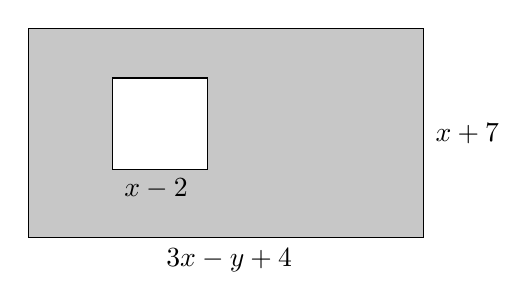
\begin{tikzpicture}[x=0.75pt,y=0.75pt,yscale=-0.75,xscale=0.75]
                        %uncomment if require: \path (0,173); %set diagram left start at 0, and has height of 173

                        %Shape: Rectangle [id:dp5990197657569669]
                        \draw  [fill={rgb, 255:red, 199; green, 199; blue, 199 }  ,fill opacity=1 ] (10,11) -- (264,11) -- (264,145.5) -- (10,145.5) -- cycle ;
                        %Shape: Rectangle [id:dp05864984865213696]
                        \draw  [fill={rgb, 255:red, 255; green, 255; blue, 255 }  ,fill opacity=1 ] (64,43) -- (125,43) -- (125,101.5) -- (64,101.5) -- cycle ;

                        % Text Node
                        \draw (70,106) node [anchor=north west][inner sep=0.75pt]    {$x-2$};
                        % Text Node
                        \draw (97,151) node [anchor=north west][inner sep=0.75pt]    {$3x-y+4$};
                        % Text Node
                        \draw (270,70.4) node [anchor=north west][inner sep=0.75pt]    {$x+7$};
                    \end{tikzpicture}
                } & \vspace{-6.2cm}\begin{mybox2}[colbacktitle=green]{Problem-solving}
                    \rmfamily
                    Use the strategy as you use if the lengths were given as number.\vspace{2mm}\\
                    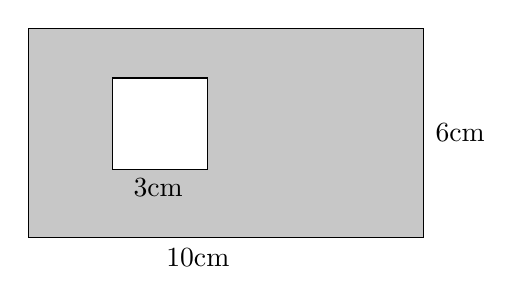
\begin{tikzpicture}[x=0.75pt,y=0.75pt,yscale=-0.75,xscale=0.75]
                        %uncomment if require: \path (0,173); %set diagram left start at 0, and has height of 173

                        %Shape: Rectangle [id:dp5990197657569669]
                        \draw  [fill={rgb, 255:red, 199; green, 199; blue, 199 }  ,fill opacity=1 ] (10,11) -- (264,11) -- (264,145.5) -- (10,145.5) -- cycle ;
                        %Shape: Rectangle [id:dp05864984865213696]
                        \draw  [fill={rgb, 255:red, 255; green, 255; blue, 255 }  ,fill opacity=1 ] (64,43) -- (125,43) -- (125,101.5) -- (64,101.5) -- cycle ;

                        % Text Node
                        \draw (76,106) node [anchor=north west][inner sep=0.75pt]    {$3$cm};
                        % Text Node
                        \draw (97,151) node [anchor=north west][inner sep=0.75pt]    {$10$cm};
                        % Text Node
                        \draw (270,70.4) node [anchor=north west][inner sep=0.75pt]    {$6$cm};
                    \end{tikzpicture}
                \end{mybox2}
            \end{tabularx}
        \end{table}
        \item A cuboid has dimensions $x+2$, $2x-1$cm and $2x+3$cm. \\ % TODO Exercise 1B - Qu. 4
              Show that the volume of the cuboid is $4x^3+12x^2+5x-6$cm$^3$.
        \item Given that $(2x+5y)(3x-y)(2x+y)=ax^3+bx^2y+cxy^2+dy^3$, where $a$, $b$, $c$ and $d$ are constants, find the values of $a$, $b$, $c$ and $d$. % TODO Exercise 1B - Qu. 5
\end{enumerate}

\exercise{}
\begin{enumerate}
    \item Expand and simplify if possible:
        \begin{tasks}(3) % TODO Exercise 1C - Qu. 1
              \task $4x+8$            % a
              \task $6x-24$           % b
              \task $20x+15$          % c
              \task $2x^2+4$          % d
              \task $4x^2+20$         % e
              \task $6x^2-18x$        % f
              \task $x^2-7x$          % g
              \task $2x^2+4x$         % h
              \task $3x^2-x$          % i
              \task $6x^2-2x$         % j
              \task $10y^2-5y$        % k
              \task $35x^2-28x$       % l
              \task $x^2+2x$          % m
              \task $3y^2+2y$         % n
              \task $4x^2+12x$        % o
              \task $5y^2-20y$        % p
              \task $9xy^2+12x^2y$    % q
              \task $6ab-2ab^2$       % r
              \task $5x^2-25xy$       % s
              \task $12x^2y+8xy^2$    % t
              \task $15y-20yz^2$      % u
              \task $12x^2-30$        % v
              \task $xy^2-x^2y$       % w
              \task $12y^2-4yx$       % x
        \end{tasks}
        \newpage
    \item Factorise:
        \begin{tasks}(3) % TODO Exercise 1C - Qu. 2
            \task $x^2+4x$           % a
            \task $2x^2+6x$          % b
            \task $x^2+11x+24$       % c
            \task $x^2+8x+12$        % d
            \task $x^2+3x-40$        % e
            \task $x^2-8x+12$        % f
            \task $x^2+5x+6$         % g
            \task $x^2-2x-24$        % h
            \task $x^2-3x-10$        % i
            \task $x^2+x-20$         % j
            \task $2x^2+5x+2$        % k
            \task $3x^2+10x-8$       % l
            \task $5x^2-16x+3$       % m
            \task $6x^2-8x-8$        % n
            \task[]
                \hspace*{-2.25cm}
                \begin{minipage}[t][][c]{0.42\textwidth}
                \vspace{-0.3cm}
                \begin{note*}{Hint}{}
                     For part $n$, take 2 out as a common factor first. For part $p$, let $y=x^2$.
                 \end{note*}
                \setcounter{taskscounter}{\getcurrentref{taskscounter}-1}
                \end{minipage}
                \vspace{-200cm}
            \task $2x^2+7x-15$       % o
            \task* $2x^4+14x+24$     % p
            \task $x^2-4$            % q
            \task* $x^2-49$          % r
            \task $4x^2-25$          % s
            \task $9x^2-25y^2$       % t
            \task $36x^2-4$          % u
            \task $2x^2-50$          % v
            \task $6x^2-10x+4$       % w
            \task $15x^2+42x-9$      % x
        \end{tasks}
    \item Factorise completely:
        \begin{tasks}(3) % TODO Exercise 1C - Qu. 3
            \task $x^3+2x$           % a
            \task $x^3-x^2+x$        % b
            \task $x^3-5x$           % c
            \task $x^3-9x$           % d
            \task $x^3-x^2-12x$      % e
            \task $x^3+11x^2+30x$    % f
            \task $x^3-7x^2+6x$      % g
            \task $x^3-64x$          % h
            \task $2x^3-5x^2-3x$     % i
            \task $2x^3+13x^2+15x$   % j
            \task $x^3-4x$           % k
            \task $3x^3+27x^2+60x$   % l
        \end{tasks}
    \item Factorise completely $x^4-y^4$. % TODO Exercise 1C - Qu. 4
        \begin{table}[!ht]
            \begin{tabularx}{\dimexpr\textwidth}{X@{\hskip10pt}p{3.5in}}
                { } & \vspace{-1.6cm}\begin{mybox2}[colbacktitle=green]{Problem-solving}
                        Watch out for terms that can be written as a function of a function: $x^4=(x^2)^2$.
                \end{mybox2}
            \end{tabularx}
            \vspace{-3mm}
        \end{table}
    \item Factorise completely $6x^3+7x^2-5x$.\hfill \textbf{(2 marks)} % TODO Exercise 1C - Qu. 5
\end{enumerate}
\begin{mybox2}[]{Challenge}
    \rmfamily Write $4x^4-13x^2+9$ as the product of four linear factors.
\end{mybox2}

\exercise{}
\begin{enumerate}
    \item Simplify
        \begin{tasks}(3) % TODO Exercise 1D - Qu. 1
            \task $x^3 \div x^{-2}$
            \task $x^5 \div x^7$
            \task $x^{\textstyle\frac{3}{2}} \times x^{\textstyle\frac{5}{2}}$
            \task $(x^2)^{\textstyle\frac{3}{2}}$
            \task $(x^3)^{\textstyle\frac{5}{3}}$
            \task $3x^{0.5} \times 4x^{-0.5}$
            \task $9x^{\textstyle\frac{2}{3}} \div 3x^{\textstyle\frac{1}{6}}$
            \task $5x^{\textstyle\frac{7}{5}} \div x^{\textstyle\frac{2}{5}}$
            \task $3x^4 \times 2x^{-5}$
            \task $\sqrt{\strut x} \times \sqrt[\textstyle{^3}]{\strut x}$
            \task $\Big(\sqrt{\strut x}\Big)^3 \times \Big(\sqrt[\textstyle{^3}]{\strut x}\Big)^4$
            \task $\cfrac{\sqrt[\textstyle{^3}]{ x}}{\sqrt{x}}$
        \end{tasks}
        
    \item Evaluate:
        \begin{tasks}(3)% TODO Exercise 1D - Qu. 2
            \task $25^{\textstyle\frac{1}{2}}$
            \task $81^{\textstyle\frac{3}{2}}$
            \task $27^{\textstyle\frac{1}{3}}$
            \task $4^{-2}$
            \task $9^{-\textstyle\frac{1}{2}}$
            \task $(-5)^{-3}$
            \task $\bigg(\cfrac{3}{4}\bigg)^0$
            \task $1296^{\textstyle\frac{3}{4}}$
            \task $\bigg(\cfrac{25}{16}\bigg)^{\textstyle\frac{3}{2}}$
            \task $\bigg(\cfrac{27}{8}\bigg)^{\textstyle\frac{2}{3}}$
            \task $\bigg(\cfrac{6}{5}\bigg)^{-1}$
            \task $\bigg(\cfrac{343}{512}\bigg)^{-\textstyle\frac{2}{3}}$
        \end{tasks}
        \newpage
        
    \item Simplify:
        \vspace{-2mm}
        \begin{tasks}(4) % TODO Exercise 1D - Qu. 3
            \task $(64x^{10})^{\textstyle\frac{1}{2}}$
            \task $\cfrac{5x^3-2x^2}{x^5}$
            \task $(125x^{12})^{\textstyle\frac{1}{3}}$
            \task $\cfrac{x+4x^3}{x^3}$
            \task $\cfrac{2x+x^2}{x^4}$
            \task $\bigg(\cfrac{4}{9}x^4\bigg)^{\textstyle\frac{3}{2}}$
            \task $\cfrac{9x^2-15x^5}{3x^3}$
            \task $\cfrac{5x+3x^2}{15x^3}$
        \end{tasks}
        
    % TODO Exercise 1D - Qu. 4
    \item \hspace*{2mm}\textbf{a}\hspace*{5mm} Find the value of $81^{\textstyle\frac{1}{4}}$.\hfill\textbf{(1 mark)}\vspace{1mm}\\
          \hspace*{2mm}\textbf{b}\hspace*{5mm} Simplify $x\Big(2x^{-\textstyle\frac{1}{3}}\Big)^4$.\hfill\textbf{(2 marks)}
     % TODO Exercise 1D - Qu. 5
    \item Given that $y=\cfrac{1}{8}x^3$ express each of the following in the form $kx^n$, where $k$ and $n$ are constants.\vspace{-2mm}
        \begin{tasks}(1)
            \task $y^{\textstyle\frac{1}{3}}$\hfill\textbf{(2 marks)}\vspace{-1mm}
            \task $\cfrac{1}{2}y^{-2}$\hfill\textbf{(2 marks)}
        \end{tasks}
\end{enumerate}

\exercise{}
\begin{enumerate}
    \item Do not use your calculator for this exercise. Simplify:
        \begin{tasks}(3) % TODO Exercise 1E - Qu. 1
            \task $\sqrt{28}$                            % a
            \task $\sqrt{72}$                            % b
            \task $\sqrt{50}$                            % c
            \task $\sqrt{32}$                            % d
            \task $\sqrt{90}$                            % e
            \task $\cfrac{\sqrt{12}}{2}$\vspace{-1mm}    % f
            \task $\cfrac{\sqrt{27}}{3}$                 % g
            \task $\sqrt{20}+\sqrt{80}$                  % h
            \task $\sqrt{200}+\sqrt{18}-\sqrt{72}$       % i
            \task $\sqrt{175}+\sqrt{63}-2\sqrt{28}$      % j
            \task $\sqrt{28}-2\sqrt{63}+\sqrt{7}$        % k
            \task $\sqrt{80}-2\sqrt{20}+3\sqrt{45}$      % l
            \task $3\sqrt{80}-2\sqrt{20}+5\sqrt{45}$     % m
            \task $\cfrac{\sqrt{44}}{\sqrt{11}}$         % n
            \task $\sqrt{12}+3\sqrt{48}+\sqrt{75}$       % o
        \end{tasks}
    \item Expand and simplify if possible:
        \begin{tasks}(3) % TODO Exercise 1E - Qu. 2
            \task $\sqrt{3}(2+\sqrt{3})$                 % a
            \task $\sqrt{5}(3-\sqrt{3})$                 % b
            \task $\sqrt{2}(4-\sqrt{5})$                 % c
            \task $(2-\sqrt{2})(3+\sqrt{5})$             % d
            \task $(2-\sqrt{3})(3-\sqrt{7})$             % e
            \task $(4+\sqrt{5})(2+\sqrt{5})$             % f
            \task $(5-\sqrt{3})(1-\sqrt{3})$             % g
            \task $(4+\sqrt{3})(2-\sqrt{3})$             % h
            \task $(7-\sqrt{11})(2+\sqrt{11})$           % i
        \end{tasks}
    \item Simplify $\sqrt{75}-\sqrt{12}$ giving your answer in the form $a\sqrt{3}$, where $a$ is an integer.\hfill\textbf{(3 marks)} % TODO Exercise 1E - Qu. 3
\end{enumerate}

\exercise{}
\begin{enumerate}
    \item Simplify:
        \begin{tasks}(4) % TODO Exercise 1F - Qu. 1
            \task $\cfrac{1}{\sqrt{5}}$                  % a
            \task $\cfrac{1}{\sqrt{11}}$                 % b
            \task $\cfrac{1}{\sqrt{2}}$                  % c
            \task $\cfrac{\sqrt{3}}{\sqrt{15}}$          % d
            \task $\cfrac{\sqrt{12}}{\sqrt{48}}$         % e
            \task $\cfrac{\sqrt{5}}{\sqrt{80}}$          % f
            \task $\cfrac{\sqrt{12}}{\sqrt{156}}$        % g
            \task $\cfrac{\sqrt{7}}{\sqrt{63}}$          % h
        \end{tasks}
    \item Rationalise the denominators and simplify:
        \begin{tasks}(5) % TODO Exercise 1F - Qu. 2
            \task $\cfrac{1}{1+\sqrt{3}}$                                % a
            \task $\cfrac{1}{2+\sqrt{5}}$                                % b
            \task $\cfrac{1}{3-\sqrt{7}}$                                % c
            \task $\cfrac{4}{3-\sqrt{5}}$                                % d
            \task $\cfrac{1}{\sqrt{5}-\sqrt{3}}$                         % e
            \task $\cfrac{3-\sqrt{2}}{4-\sqrt{5}}$                       % f
            \task $\cfrac{5}{2+\sqrt{5}}$                                % g
            \task $\cfrac{5\sqrt{2}}{\sqrt{8}-\sqrt{7}}$                 % h
            \task $\cfrac{11}{3+\sqrt{11}}$                              % i
            \task $\cfrac{\sqrt{3}-\sqrt{7}}{\sqrt{3}+\sqrt{7}}$         % j
            \task $\cfrac{\sqrt{17}-\sqrt{11}}{\sqrt{17}+\sqrt{11}}$     % k
            \task $\cfrac{\sqrt{41}+\sqrt{29}}{\sqrt{41}-\sqrt{29}}$     % l
            \task $\cfrac{\sqrt{2}-\sqrt{3}}{\sqrt{3}-\sqrt{2}}$         % m
        \end{tasks}
    \setcounter{enumi}{3}
    \newpage
    \item Simplify $\cfrac{3-2\sqrt{5}}{\sqrt{5}-1}$     giving you answer in the    \\ % TODO Exercise 1F - Qu. 4
          \indent form $p+q\sqrt{5}$, where $p$ and $q$ are rational                 \\
          number.\hspace*{40mm}\textbf{(4 marks)}\vspace{-4mm}                       \\
        \begin{table}[!ht]
            \begin{tabularx}{\dimexpr\textwidth}{X@{\hskip10pt}p{3.5in}}
                { } & \vspace{-3cm}\begin{mybox2}[colbacktitle=green]{Problem-solving}
                        You can check that you answer is in the correct form but writing down the values of p and q and check that they are rational numbers.
                \end{mybox2}
            \end{tabularx}
            \vspace{-8mm}
        \end{table}
\end{enumerate}



\exercise{Mixed Exercise 1}
\begin{enumerate}
    \item Simplify:
        \begin{tasks}(4) % TODO Mixed Exercise - Qu. 1
            \task $y^3 \times y^5$                    % a
            \task $3x^2 \times 2x^5$                  % b
            \task $(4x^2)^3$                          % c
            \task $4b^2 \times 3b^3 \times b^4$       % d
        \end{tasks}
        
    \item Expand and simplify if possible:
        \begin{tasks}(3) % TODO Mixed Exercise - Qu. 2
            \task $(x+3)(x-5)$
            \task $(2x-7)(3x+1)$
            \task $(2x+5)(3x-y+2)$
        \end{tasks}
        
    \item Expand and simplify if possible:
        \begin{tasks}(3) % TODO Mixed Exercise - Qu. 3
            \task $x(x+4)(x-1)$                       % a
            \task $(x+2)(x-3)(x+7)$                   % b
            \task $(2x+3)(x-2)(3x-1)$                 % c
        \end{tasks}
        
    \item Expand the brackets: \vspace{3mm}\\\hspace*{1mm} % TODO Mixed Exercise - Qu. 4
        \begin{enumerate*}[label=\textbf{\alph*}]
            \item $3(5y+4)$                 \hspace*{5mm}    % a
            \item $5x^2(3-5x+2x^2)$         \hspace*{5mm}    % b
            \item $5x(2x+3)-2x(1-3x)$       \hspace*{5mm}    % c
            \item $3x^2(1+3x)-2x(3x-2)$                      % d
        \end{enumerate*}
        
    \item Factorise these expressions completely:
        \begin{tasks}(4) % TODO Mixed Exercise - Qu. 5
            \task $3x^2+4x$             % a
            \task $4y^2+10y$            % b
            \task $x^2+xy+xy^2$         % c
            \task $8xy^2+10x^2y$        % d
        \end{tasks}
        
    \item Factorise:
        \begin{tasks}(4) % TODO Mixed Exercise - Qu. 6
            \task $x^2+3x+2$            % a
            \task $3x^2+6x$             % b
            \task $x^2-2x-35$           % c
            \task $2x^2-x-3$            % d
            \task $5x^2-13x-6$          % e
            \task $6-5x-x^2$            % f
        \end{tasks}
        
    \item Factorise:
        \begin{tasks}(4)% TODO Mixed Exercise - Qu. 7
            \task $2x^3+6x$            % a
            \task $x^3-36x$            % b
            \task $2x^3+7x^2-15x$      % c
        \end{tasks}
        
    \item Simplify: \vspace{-2mm}
        \begin{tasks}(4) % TODO Mixed Exercise - Qu. 8
            \task $9x^3 \div 3x^{-3}$
            \task $\big(4^{\textstyle\frac{3}{2}}\big)^{\textstyle\frac{1}{3}}$
            \task $3x^{-2} \times 2x^4$
            \task $3x^{\textstyle\frac{1}{3}} \div 6x^{\textstyle\frac{2}{3}}$
        \end{tasks}
        
    \item Evaluate: \vspace{-2mm}
        \begin{tasks}(4) % TODO Mixed Exercise - Qu. 9
            \task $\cfrac{3}{\sqrt{63}}$
            \task $\bigg(\cfrac{225}{289}\bigg)^{\textstyle\frac{3}{2}}$
        \end{tasks}
        
    \item Simplify: \vspace{-2mm} % TODO Mixed Exercise - Qu. 10
        \begin{tasks}(4)
            \task $\cfrac{3}{\sqrt{63}}$                % a
            \task $\sqrt{20}+2\sqrt{45}-\sqrt{80}$      % b
        \end{tasks}
        
    % TODO Mixed Exercise - Qu. 11
    \item \hspace*{2mm}\textbf{a}\hspace*{5mm} Find the value of $35x^2+2x-48$.\vspace{1mm}\\
          \hspace*{2mm}\textbf{b}\hspace*{5mm} By factorising the expression, show that your answer to part \textbf{a} can be written as the product of two \linebreak\hspace*{10.5mm}prime factors.
          
    \item Expand and simplify if possible:
        \begin{tasks}(3) % TODO Mixed Exercise - Qu. 12
            \task $\sqrt{2}(3+\sqrt{5})$
            \task $(2-\sqrt{5})(5+\sqrt{3})$
            \task $(6-\sqrt{2})(4-\sqrt{7})$
        \end{tasks}
        
    \item Rationalise the denominator and simplify: \vspace{-2mm}
        \begin{tasks}(6) % TODO Mixed Exercise - Qu. 13
            \task $\cfrac{1}{\sqrt{3}}$
            \task $\cfrac{1}{\sqrt{2}-1}$
            \task $\cfrac{3}{\sqrt{3}-2}$
            \task $\cfrac{\sqrt{23}-\sqrt{37}}{\sqrt{23}+\sqrt{37}}$
            \task $\cfrac{1}{(2+\sqrt{3})^2}$
            \task $\cfrac{1}{(4-\sqrt{7})^2}$
        \end{tasks}
        
    % TODO Mixed Exercise - Qu. 14
    \item \hspace*{2mm}\textbf{a}\hspace*{5mm} Given that $x^3-x^2-17x-15=(x+3)(x^2+bx+c)$, where $b$ and $c$ are constants, work out the \\\hspace*{9mm} values of $b$ and $c$.\vspace{1mm}\\
          \hspace*{2mm}\textbf{b}\hspace*{5mm} Hence, fully factorise $x^3-x^2-17x-15$.
    \newpage

    % TODO Mixed Exercise - Qu. 15
    \item Given that $y=\cfrac{1}{64}x^3$ express each of the following in the form $kn^n$, where $k$ and $n$ are constants. \vspace{-2mm}
        \begin{tasks}(1)
            \task $y^{\textstyle\frac{1}{3}}$
            \task $4y^{-1}$
        \end{tasks}
        \vspace{-4mm}
        
    % TODO Mixed Exercise - Qu. 16
    \item Show that $\cfrac{5}{\sqrt{75}-\sqrt{50}}$ can be written in the form $\sqrt{a}+\sqrt{b}$, where $a$ and $b$ are integers. \hfill\textbf{(5 marks)}
    
    % TODO Mixed Exercise - Qu. 17
    \item Expand and simplify $(\sqrt{11}-5)(5-\sqrt{11})$. \hfill\textbf{(2 marks)}
    
    % TODO Mixed Exercise - Qu. 18
    \item Factorise completely $x-64x^3$. \hfill\textbf{(3 marks)}
    
    % TODO Mixed Exercise - Qu. 19
    \item Express $27^{2x+1}$ in the form $3^y$, stating $y$ in terms of $x$. \hfill\textbf{(2 marks)}
    
    % TODO Mixed Exercise - Qu. 20
    \item \vspace{-2mm}Solve the equation $8+x\sqrt{12}=\cfrac{8x}{\sqrt{3}}$\\
        Give your answer in the form $a\sqrt{b}$, where $a$ and $b$ are integers.\hfill\textbf{(4 marks)}
    % TODO Mixed Exercise - Qu. 21
    \item A rectangle has a length of $(1+\sqrt{3})$cm and area of $\sqrt{12}$cm$^2$.\\
          Calculate the width of the rectangle in cm.\\
          Express you answer in the form $a+b\sqrt{3}$, where $a$ and $b$ are integers to be found.
    
    % TODO Mixed Exercise - Qu. 22
    \item Show that $\cfrac{(2-\sqrt{x})^2}{\sqrt{x}}$ can be written as $4x^{-\textstyle\frac{1}{2}}-4+x^{\textstyle\frac{1}{2}}$. \hfill\textbf{(2 marks)}
    
    % TODO Mixed Exercise - Qu. 23
    \item Given $243\sqrt{3}=3^a$, find the value of $a$. \hfill\textbf{(3 marks)}
    
    % TODO Mixed Exercise - Qu. 24
    \item \vspace{-1.5mm}Given that $\cfrac{4x^3+x^{\textstyle\frac{5}{2}}}{\sqrt{x}}$ can be written in the form $4x^a+x^b$, write down the value of $a$ and\\ the value of $b$. \hfill\textbf{(2 marks)}
\end{enumerate}


% TODO Mixed Exercise - Challenge
\begin{mybox2}[colbacktitle=green]{Challenge}
    \rmfamily
    \begin{enumerate}[label=\textbf{\alph*}]
        \item Simplify $\Big(\sqrt{\strut a}+\sqrt{\strut b}\Big)\Big(\sqrt{\strut a}-\sqrt{\strut b}\Big)$
        \item \vspace{-2mm}Hence show that $\cfrac{1}{\sqrt{1}+\sqrt{2}}+\cfrac{1}{\sqrt{2}+\sqrt{3}}+\cfrac{1}{\sqrt{3}+\sqrt{4}}+...+\cfrac{1}{\sqrt{24}+\sqrt{25}}=4$
    \end{enumerate}

\end{mybox2}







\end{document}
